\section{Conclusion}

All three approaches maintain a high speed-up while still offering a high coverage.

For each ECU, the same scan as in \autoref{sec:introduction} was executed, they differ only in the use of the new implementations. As \autoref{fig:durations-diff} illustrates, the speed-up is severe.

\begin{figure}[h]
    \centering
    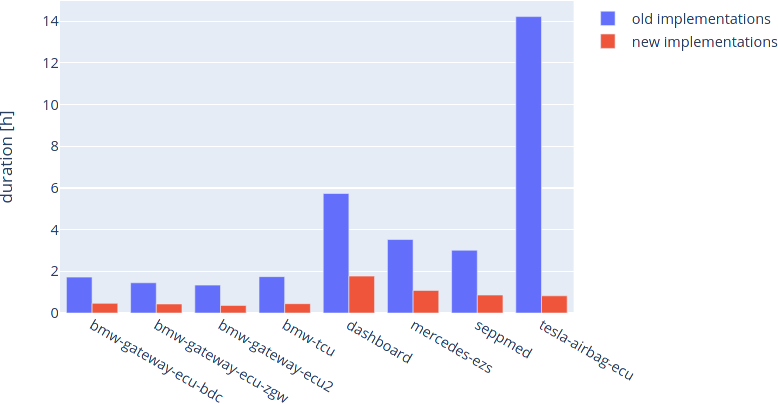
\includegraphics[width=1\textwidth]{durations-diff}
    \caption{Observed runtimes for a UDS scan with new implementations.}
    \label{fig:durations-diff}
\end{figure}

The use of information within the same scan (approach 1) is applicable to scans of services multiple fields, as it is the case with the RC service that has the type and identifier field. This results in a high scan time for this service and thus a high potential time savings. However, if an identifier is not recognized in the first scan, it will not be recognized in the next scans as well.

The biggest problem with reducing the scan range (approach 2) is the newly added random factor. The coverage can be great for one scan, but low for the next one. This would require performing multiple scans using the new implementation to ensure that most identifiers were found.

Avoiding scanning unsupported services (approach 3) is the safest way to save time. It is unlikely that identifiers will be missed, but the speed gain can still be very high.

Nevertheless, all three approaches are not able to provide a 100\% coverage. 
If a coverage of 100\% is desired, a full scan might be the preferred solution, even if it takes much longer. This may be acceptable, ff this scan will be executed only once. For fast results and good, but possibly not complete coverage, the new implementation should be preferred. It depends on the use case.
